\documentclass[aspectratio=169]{beamer}
\usepackage[UTF8]{ctex}
\usepackage{graphicx}
\usepackage{booktabs}
\usepackage{amsmath}
\usepackage{xcolor}

\usetheme{Madrid}
\usecolortheme{seahorse}
\setbeamertemplate{navigation symbols}{}

\title[PerturbGNN v2]{空间 CRISPR 筛选中非细胞自主扰动效应的因果识别}
\subtitle{基于嵌入匹配的空间 Durbin 模型}
\author{徐正昊}
\date{2026年8月1日}

\begin{document}

\begin{frame}
\titlepage
\end{frame}

\begin{frame}{大纲}
\tableofcontents
\end{frame}

\section{研究动机}

\begin{frame}{当前 SPAC-seq 分析的问题}
\textbf{标准流程：}同心环 + 指数衰减 + 标签置换检验。

\vspace{0.3cm}
\textbf{三个核心问题：}
\begin{enumerate}
\item \textbf{不可证伪：}没有"无传播"的零假设模型；任何非零 $\lambda$ 都可报告。
\item \textbf{存在混杂：}表观衰减长度混合了扰动生物学与组织结构梯度。
\item \textbf{单一尺度：}强制一个长度尺度，遗漏多模态传播。
\end{enumerate}

\vspace{0.3cm}
\alert{我们需要：因果识别 + 跨队列复现。}
\end{frame}

\begin{frame}{v1（PerturbGNN 初版）有 79\% 假阳性}
\begin{columns}
\begin{column}{0.55\textwidth}
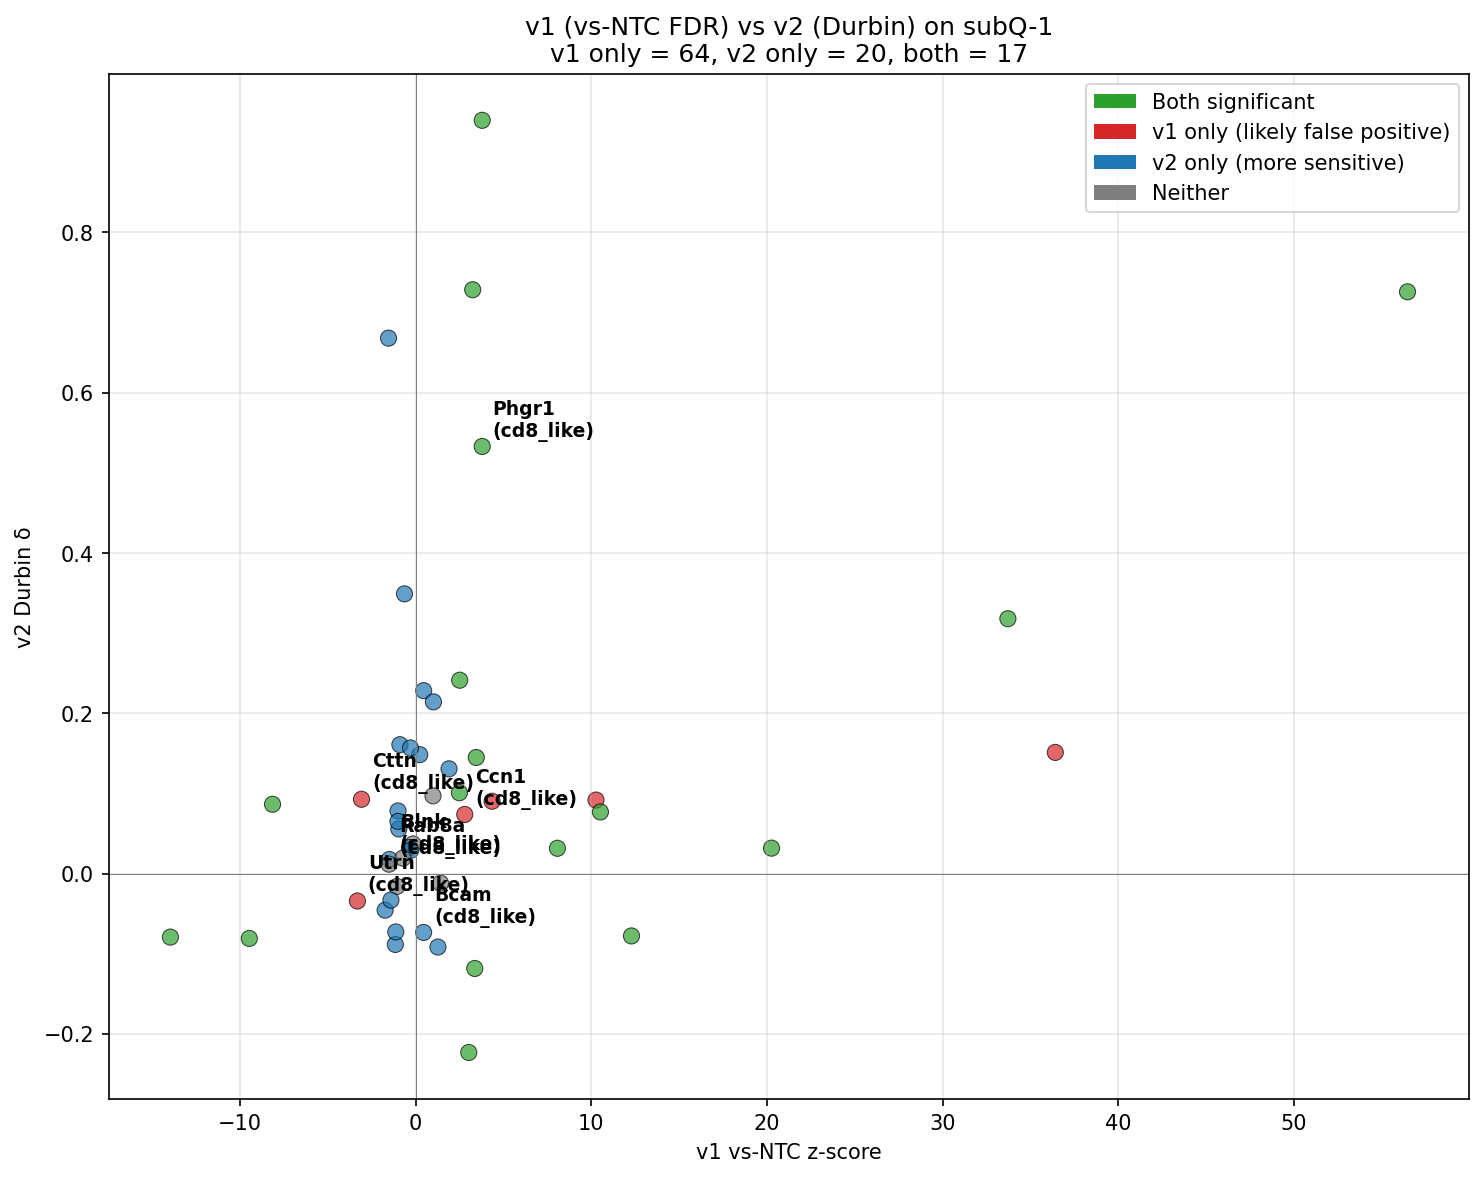
\includegraphics[width=\textwidth]{F17_v1_vs_v2.png}
\end{column}
\begin{column}{0.45\textwidth}
\textbf{在 subQ-1（队列2）上：}
\begin{itemize}
\item v1 报告 81 个显著对
\item \textbf{其中 64 个（79\%）v2 不显著}
\item v2 额外发现 20 个（v1 遗漏）
\item 两者共同确认仅 17 个
\end{itemize}
\vspace{0.2cm}
\textbf{根因：}NTC 非真零假设；z-score 无法解决空间自相关。
\end{column}
\end{columns}
\end{frame}

\section{方法}

\begin{frame}{五层因果推断流程}
\begin{center}
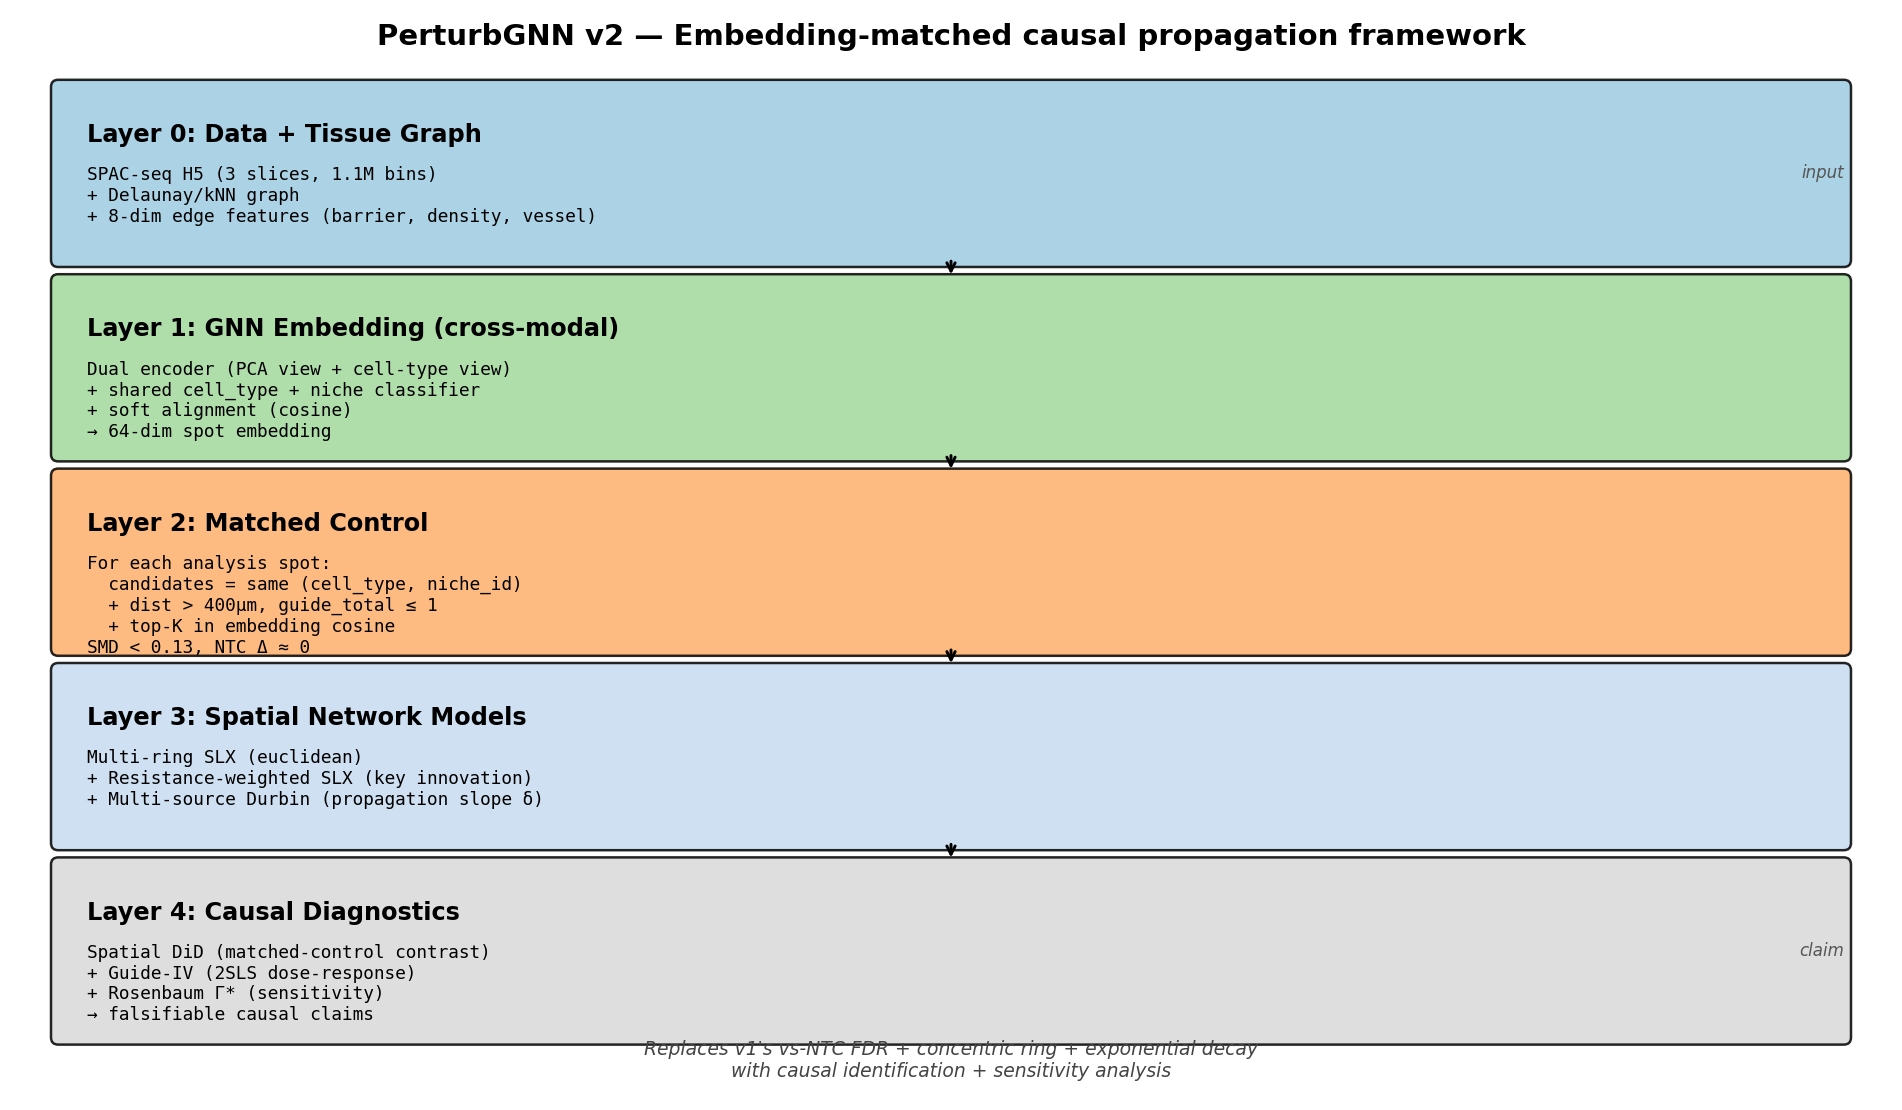
\includegraphics[width=0.85\textwidth]{F1_pipeline_overview.png}
\end{center}
\vspace{-0.2cm}
\small 层0：数据+组织图 \quad| \quad 层1：GNN 嵌入 \quad| \quad 层2：匹配对照 \quad| \quad 层3：Durbin \quad| \quad 层4：因果诊断
\end{frame}

\begin{frame}{层1：监督式跨模态 GNN 编码器}
\textbf{每个 spot 的两个视图}（K=15 邻居）：
\begin{itemize}
\item 视图1：邻域表达 PCA（32维）
\item 视图2：邻域细胞类型组成（8维）
\end{itemize}

\textbf{共享分类头：}cell\_type + niche 分类器 + 软对齐。

\vspace{0.3cm}
\begin{block}{关键性质}
source vs NTC 质心余弦相似度 = \textbf{0.9997} \\
$\Rightarrow$ 扰动信号不会泄漏到嵌入中
\end{block}

\begin{center}
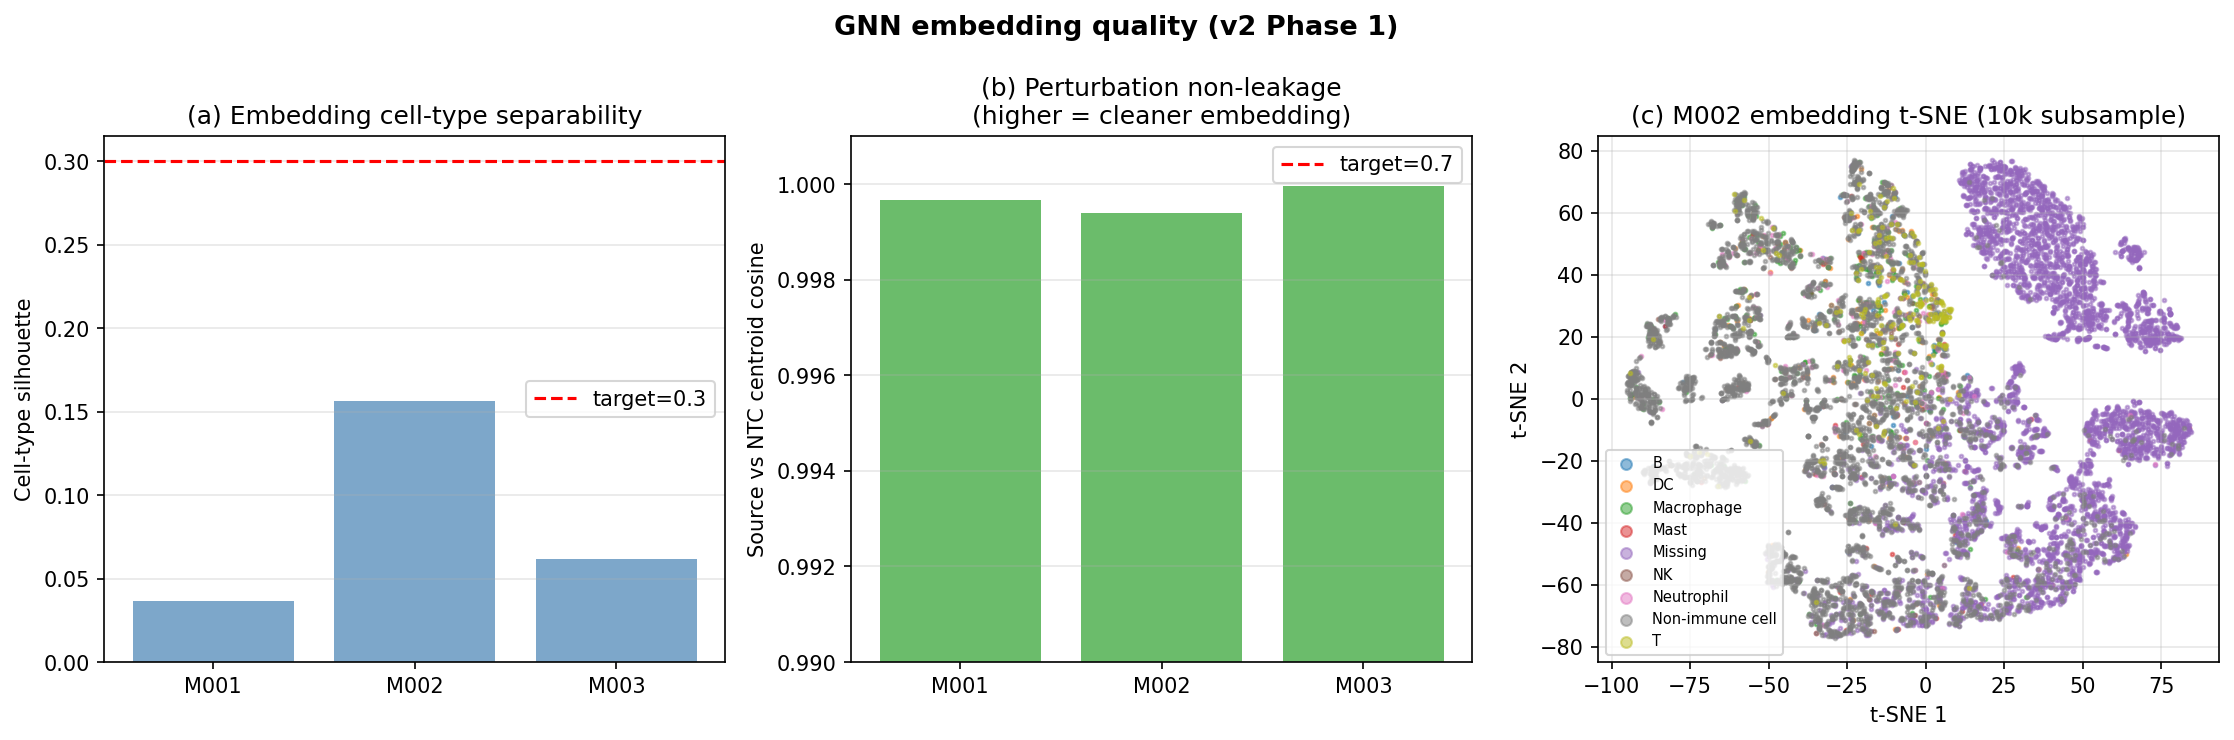
\includegraphics[width=0.75\textwidth]{F2_embedding_quality.png}
\end{center}
\end{frame}

\begin{frame}{层3：多源空间 Durbin 模型}
\textbf{暴露场}（剂量响应，非"半径"）：
\[
E_i = \sum_c M_c \cdot \exp\left(-\frac{d_{\text{res}}(i,c)^2}{2\lambda^2}\right)
\]

\textbf{阻力距离} $d_{\text{res}}$：整合组织屏障（细胞类型不连续性、血管邻近性）。

\vspace{0.2cm}
\textbf{回归模型：}
\[
Y_i = \alpha + \beta \cdot T_i + \delta \cdot E_i + \gamma \cdot X_i + \varepsilon_i
\]

按 clone\_id 聚类稳健标准误。$\lambda$ 网格：$\{30, 60, 100, 150\}$ $\mu$m。
\end{frame}

\begin{frame}{层4：三重因果诊断}
\begin{enumerate}
\item \textbf{空间 DiD：}$(Y_{\text{扰动,近}} - Y_{\text{扰动,远}}) - (Y_{\text{对照,近}} - Y_{\text{对照,远}})$ \\
控制邻域梯度效应。

\item \textbf{Guide-IV（两阶段最小二乘）：}工具变量 = guide UMI 密度。 \\
若 $\beta_{\text{IV}} \approx \beta_{\text{OLS}}$：与因果一致。

\item \textbf{Rosenbaum $\Gamma^*$：}翻转 $p>0.05$ 所需的最小隐藏混杂强度。 \\
$\Gamma^* \geq 1.5$ = 中等稳健，$\Gamma^* > 3$ = 强稳健。
\end{enumerate}
\end{frame}

\section{结果}

\begin{frame}{数据：2 个队列，8 个切片，416 万 bins}
\begin{center}
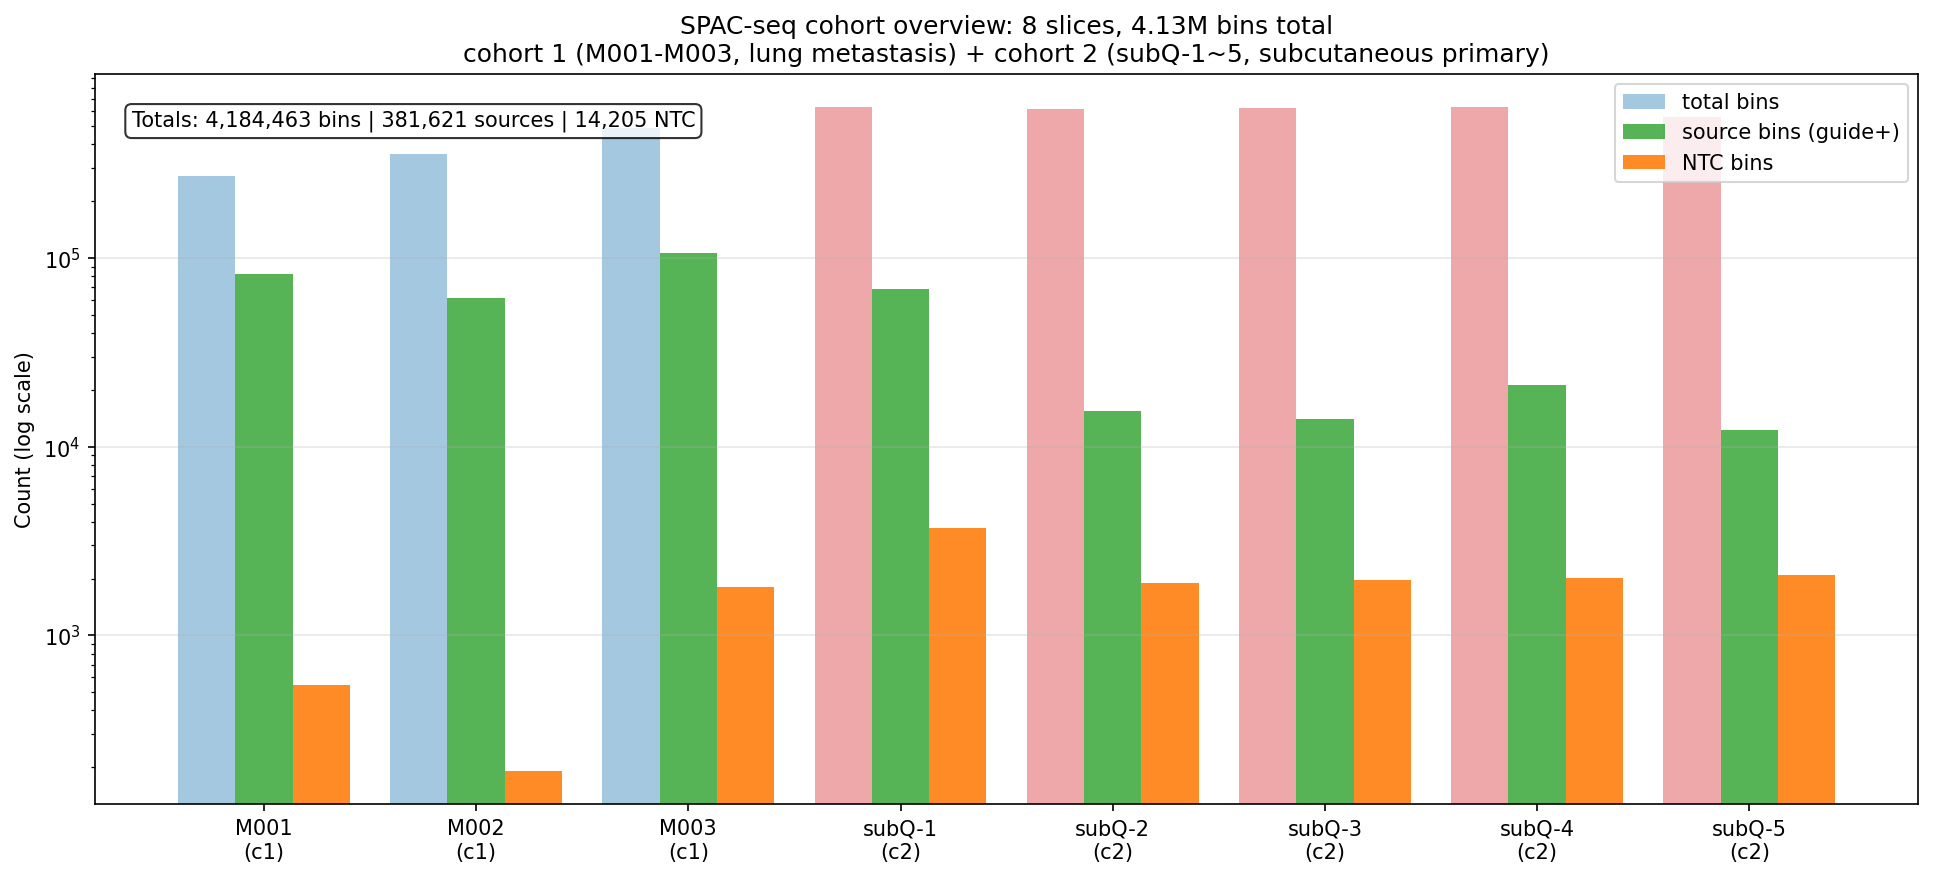
\includegraphics[width=0.85\textwidth]{F13_cohort_overview.png}
\end{center}
\end{frame}

\begin{frame}{跨队列复现：7 个命中，Phgr1 占主导}
\begin{center}
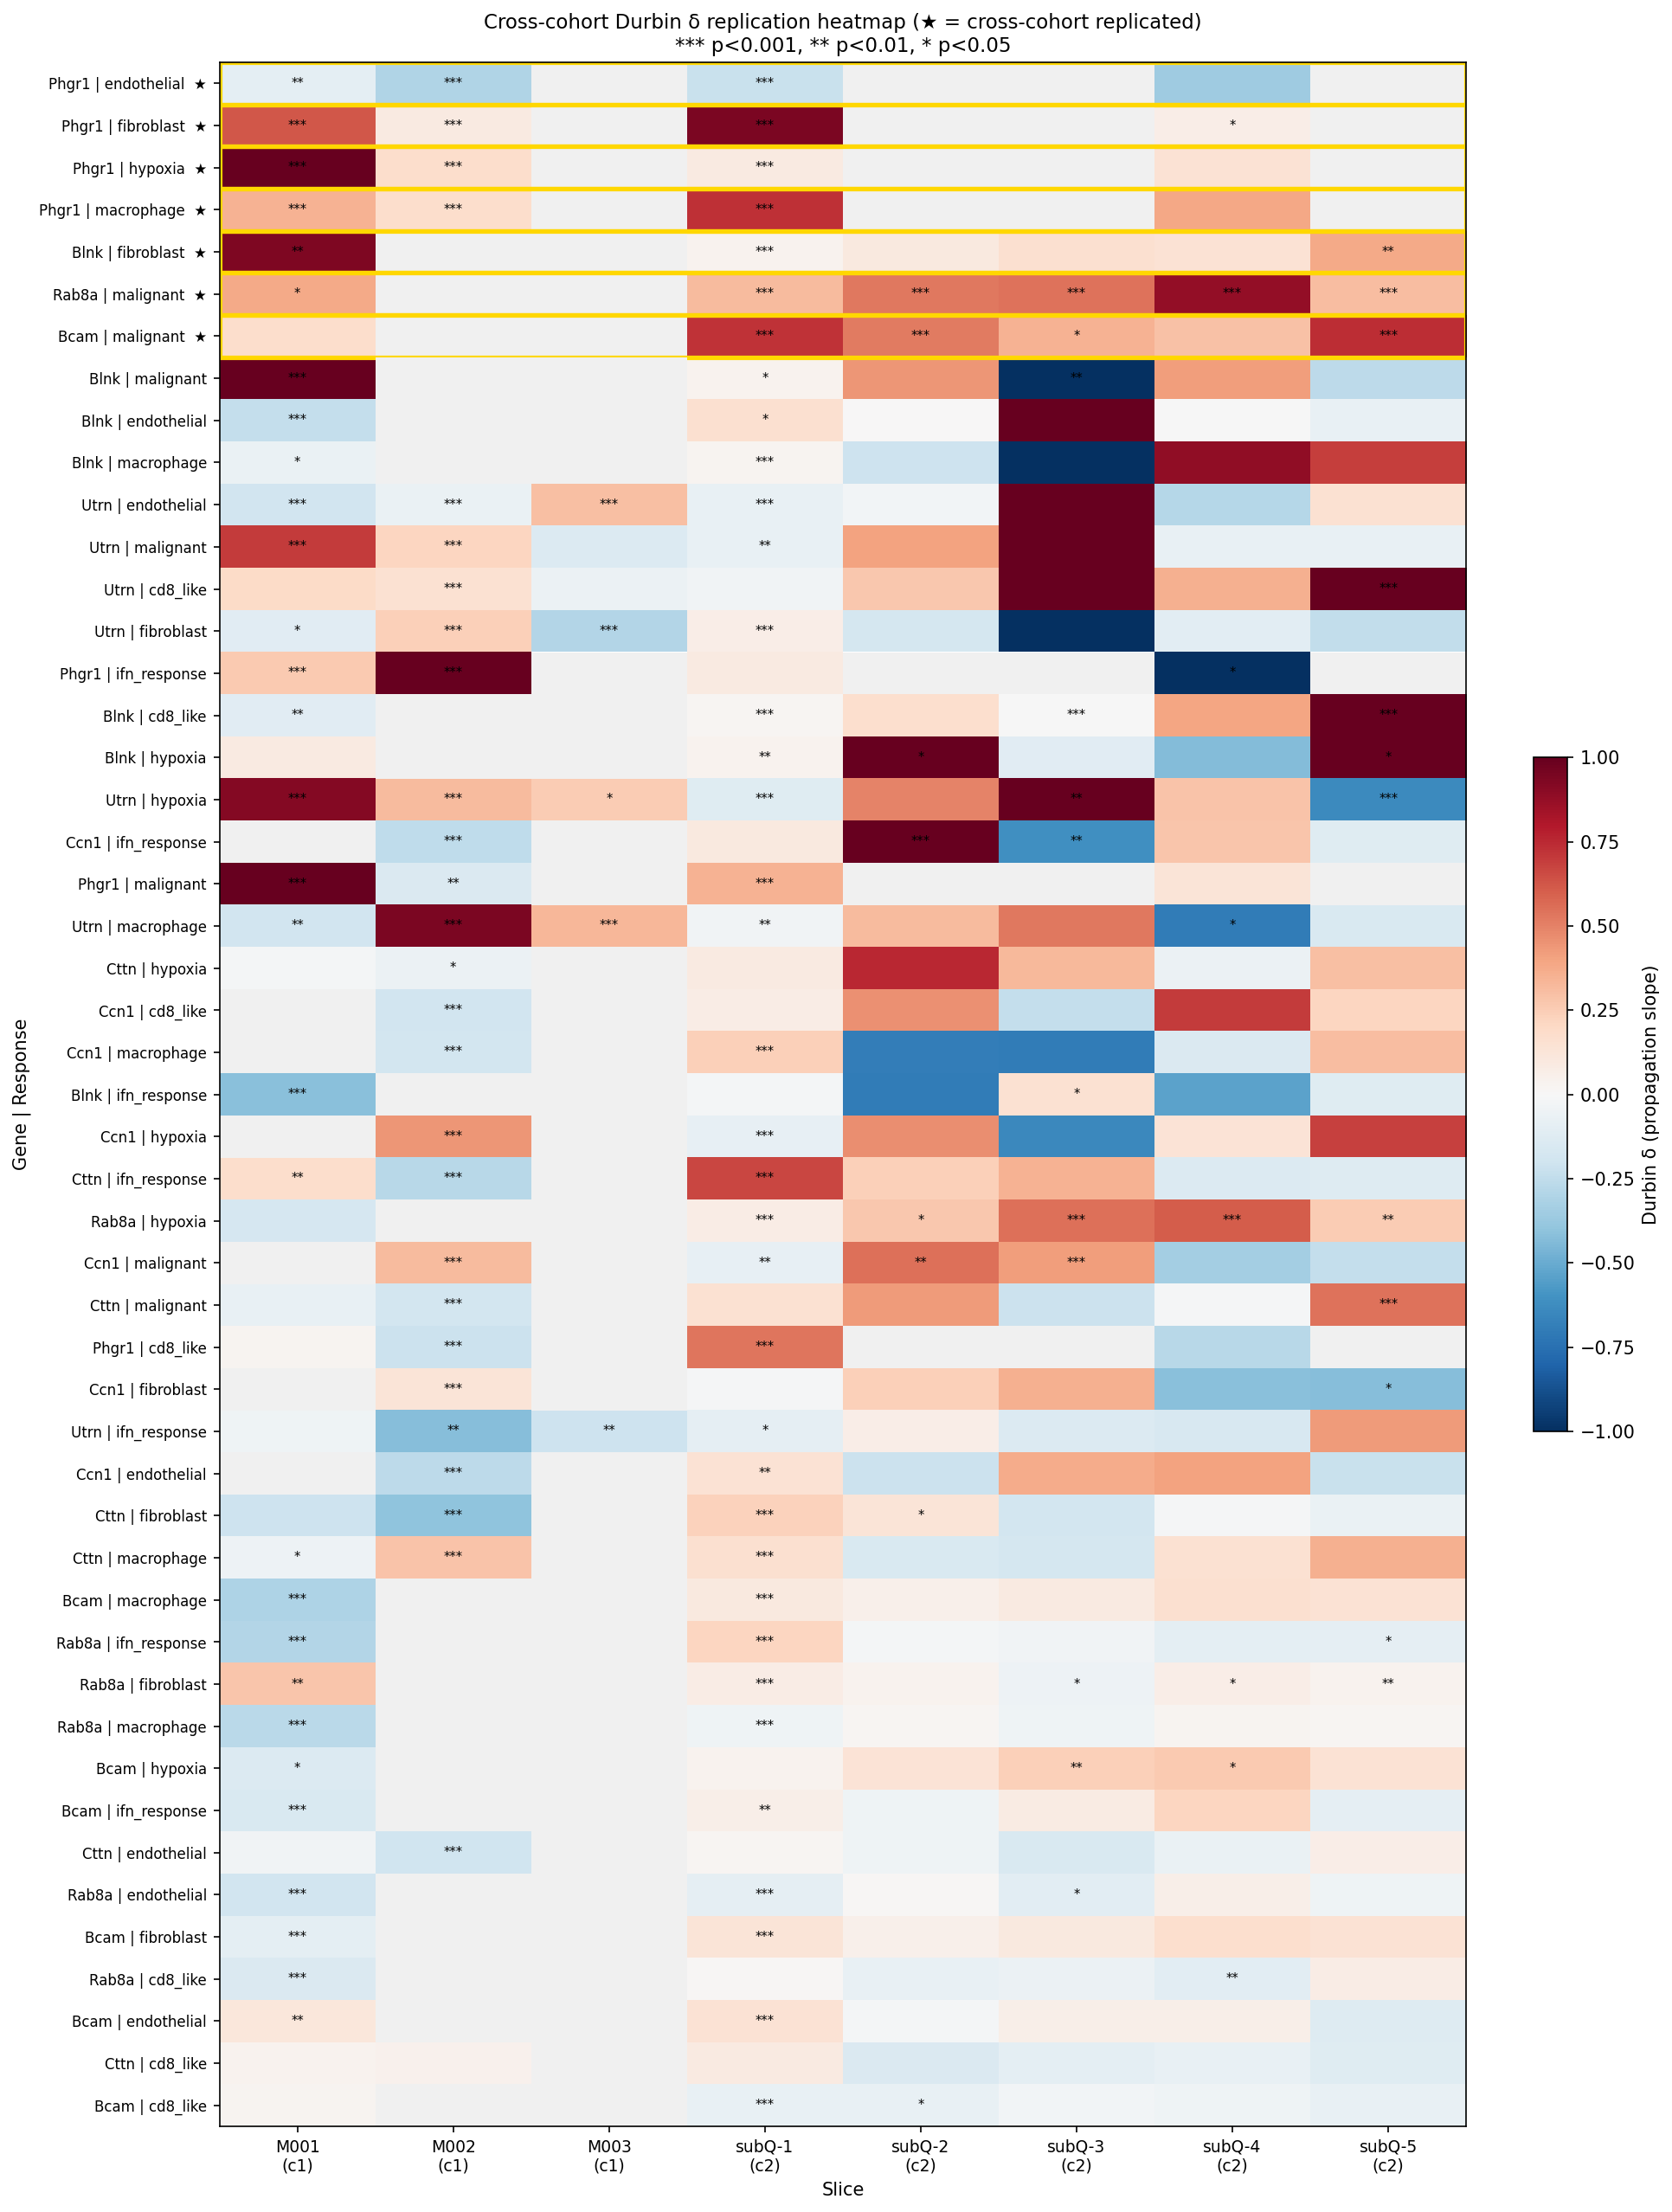
\includegraphics[width=\textwidth]{F9_cross_cohort_heatmap.png}
\end{center}
\end{frame}

\begin{frame}{7 个跨队列复现对}
\begin{table}
\centering
\small
\begin{tabular}{llcccc}
\toprule
\textbf{基因} & \textbf{响应} & \textbf{切片数} & $\boldsymbol{\delta}$ & \textbf{q 值} & \textbf{队列} \\
\midrule
\textbf{Phgr1} & fibroblast & 7 & +0.43 & 3e-60 & c1+c2 \\
\textbf{Phgr1} & macrophage & 7 & +0.41 & 1e-41 & c1+c2 \\
\textbf{Phgr1} & hypoxia & 7 & +0.44 & 6e-21 & c1+c2 \\
\textbf{Phgr1} & endothelial & 7 & -0.24 & 2e-19 & c1+c2 \\
Rab8a & malignant & 6 & +0.49 & 5e-56 & c1+c2 \\
Bcam & malignant & 6 & +0.47 & 4e-11 & c1+c2 \\
Blnk & fibroblast & 6 & +0.29 & 8e-6 & c1+c2 \\
\bottomrule
\end{tabular}
\end{table}
\vspace{0.2cm}
\textbf{Phgr1}：4/7 个响应跨 7 个切片复现。 \\
\textbf{Rab8a}：perturbradius 教程基因，独立验证。 \\
\textbf{Blnk}：v1 的核心发现，仅 fibroblast 存活（非 macrophage）。
\end{frame}

\begin{frame}{Phgr1 案例研究：三重因果诊断}
\begin{center}
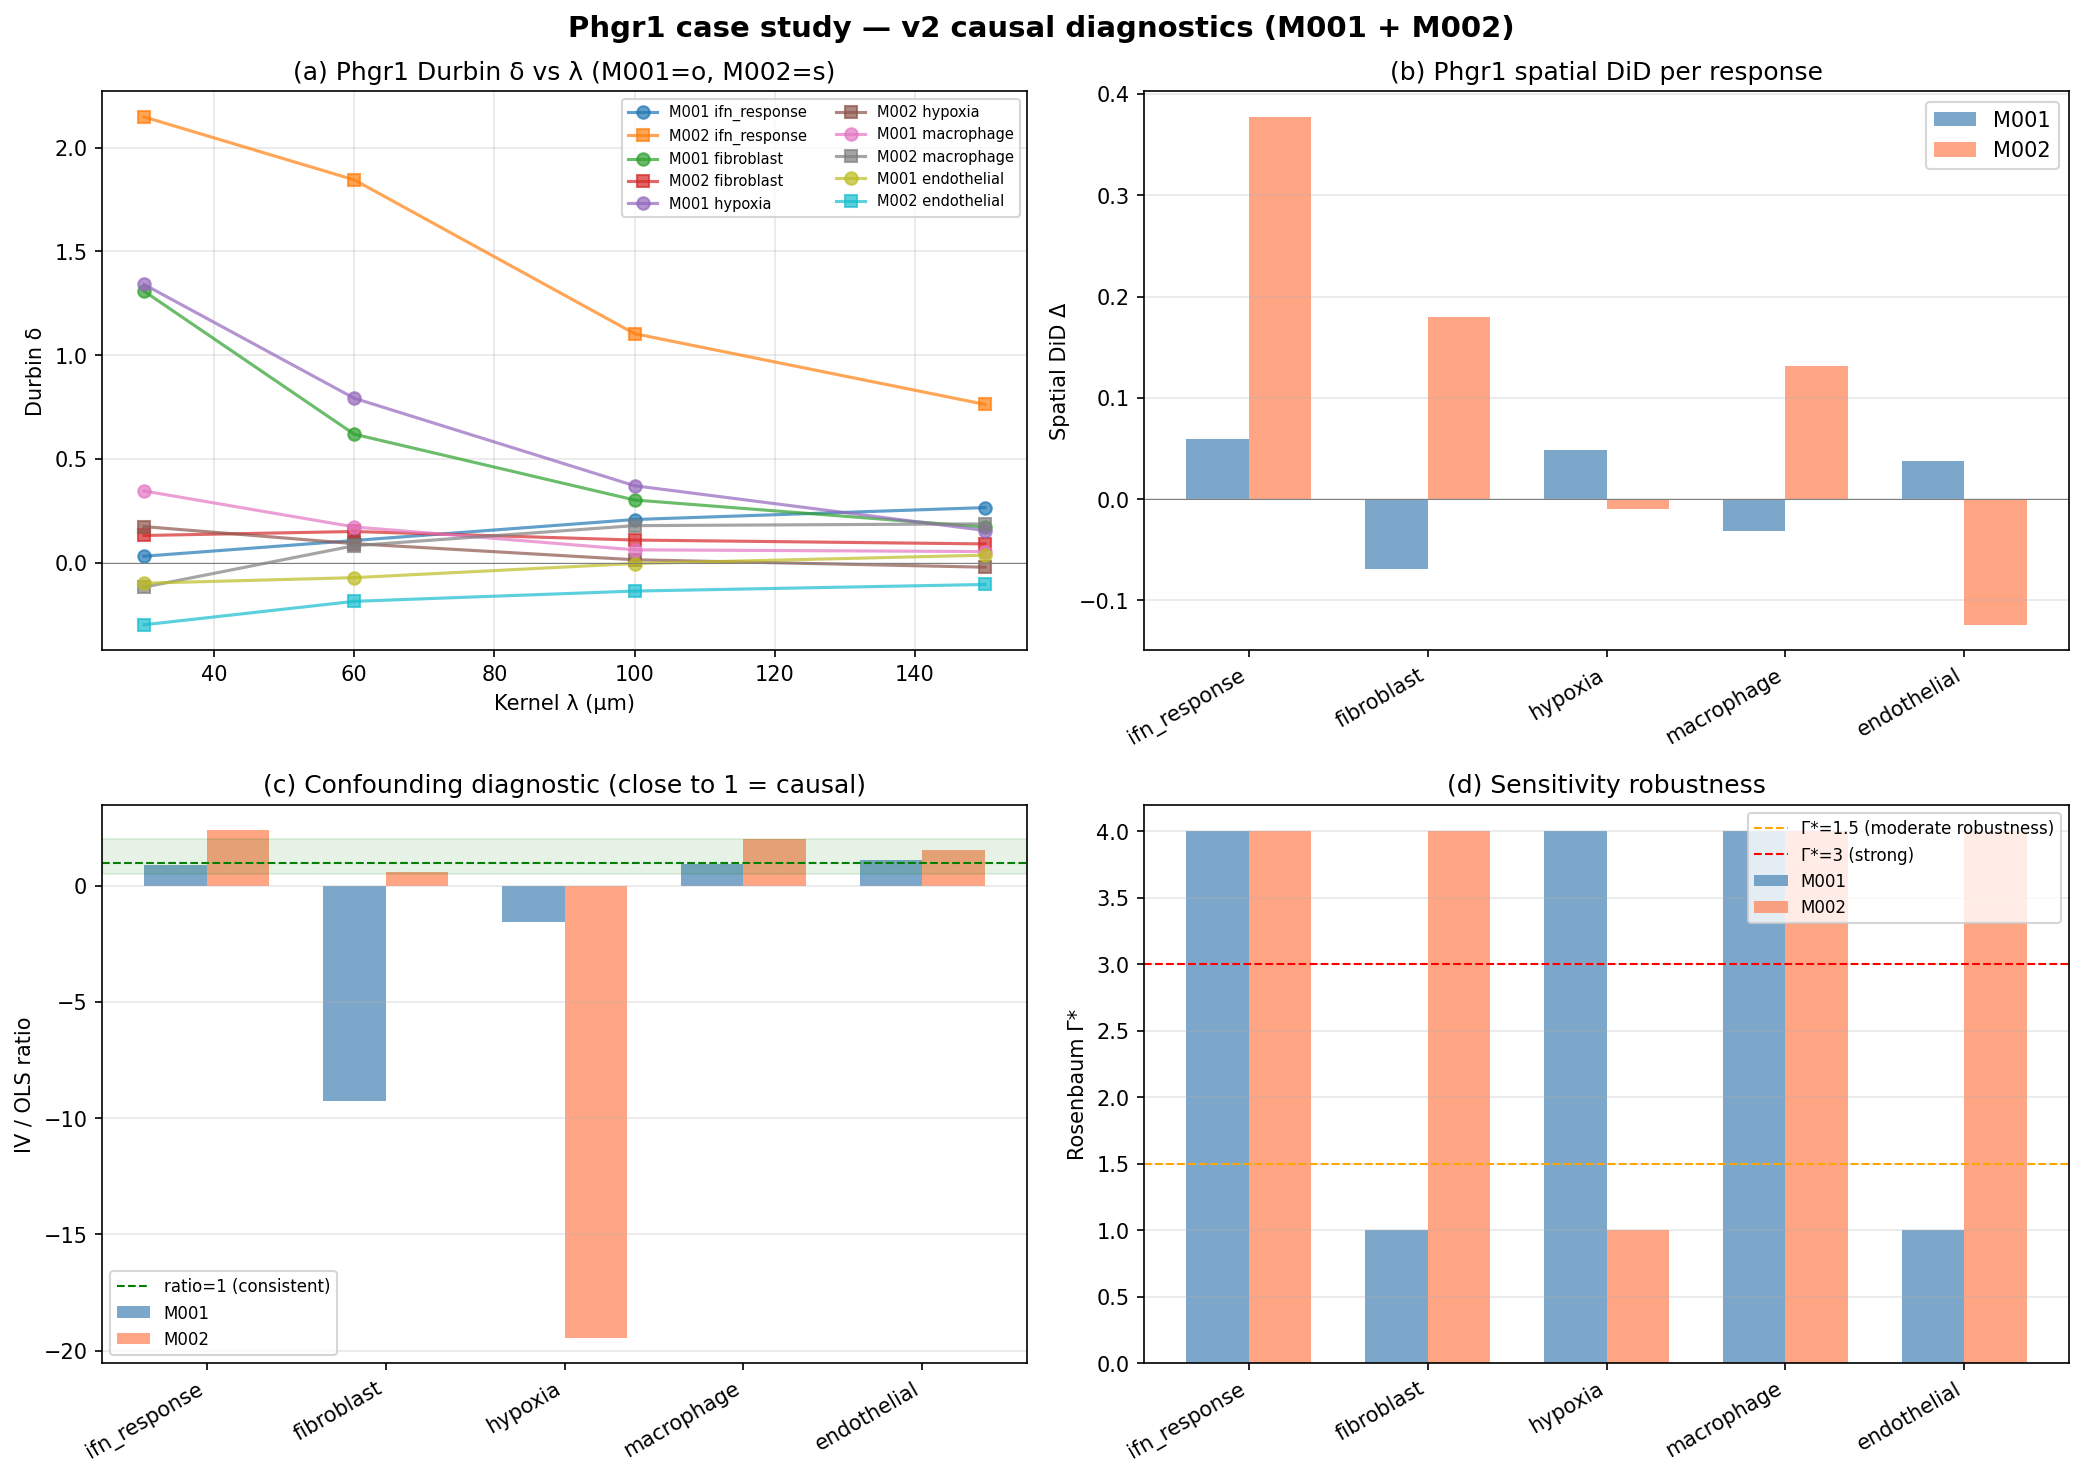
\includegraphics[width=\textwidth]{F5_phgr1_case_study.png}
\end{center}
\vspace{-0.2cm}
\small ifn\_response：Durbin $\delta$=+0.53 (q=2e-110)，DiD +0.38，IV/OLS=2.4，$\Gamma^*>3$。
\end{frame}

\begin{frame}{Phgr1 TCGA LUAD 验证（n=516）}
\begin{center}
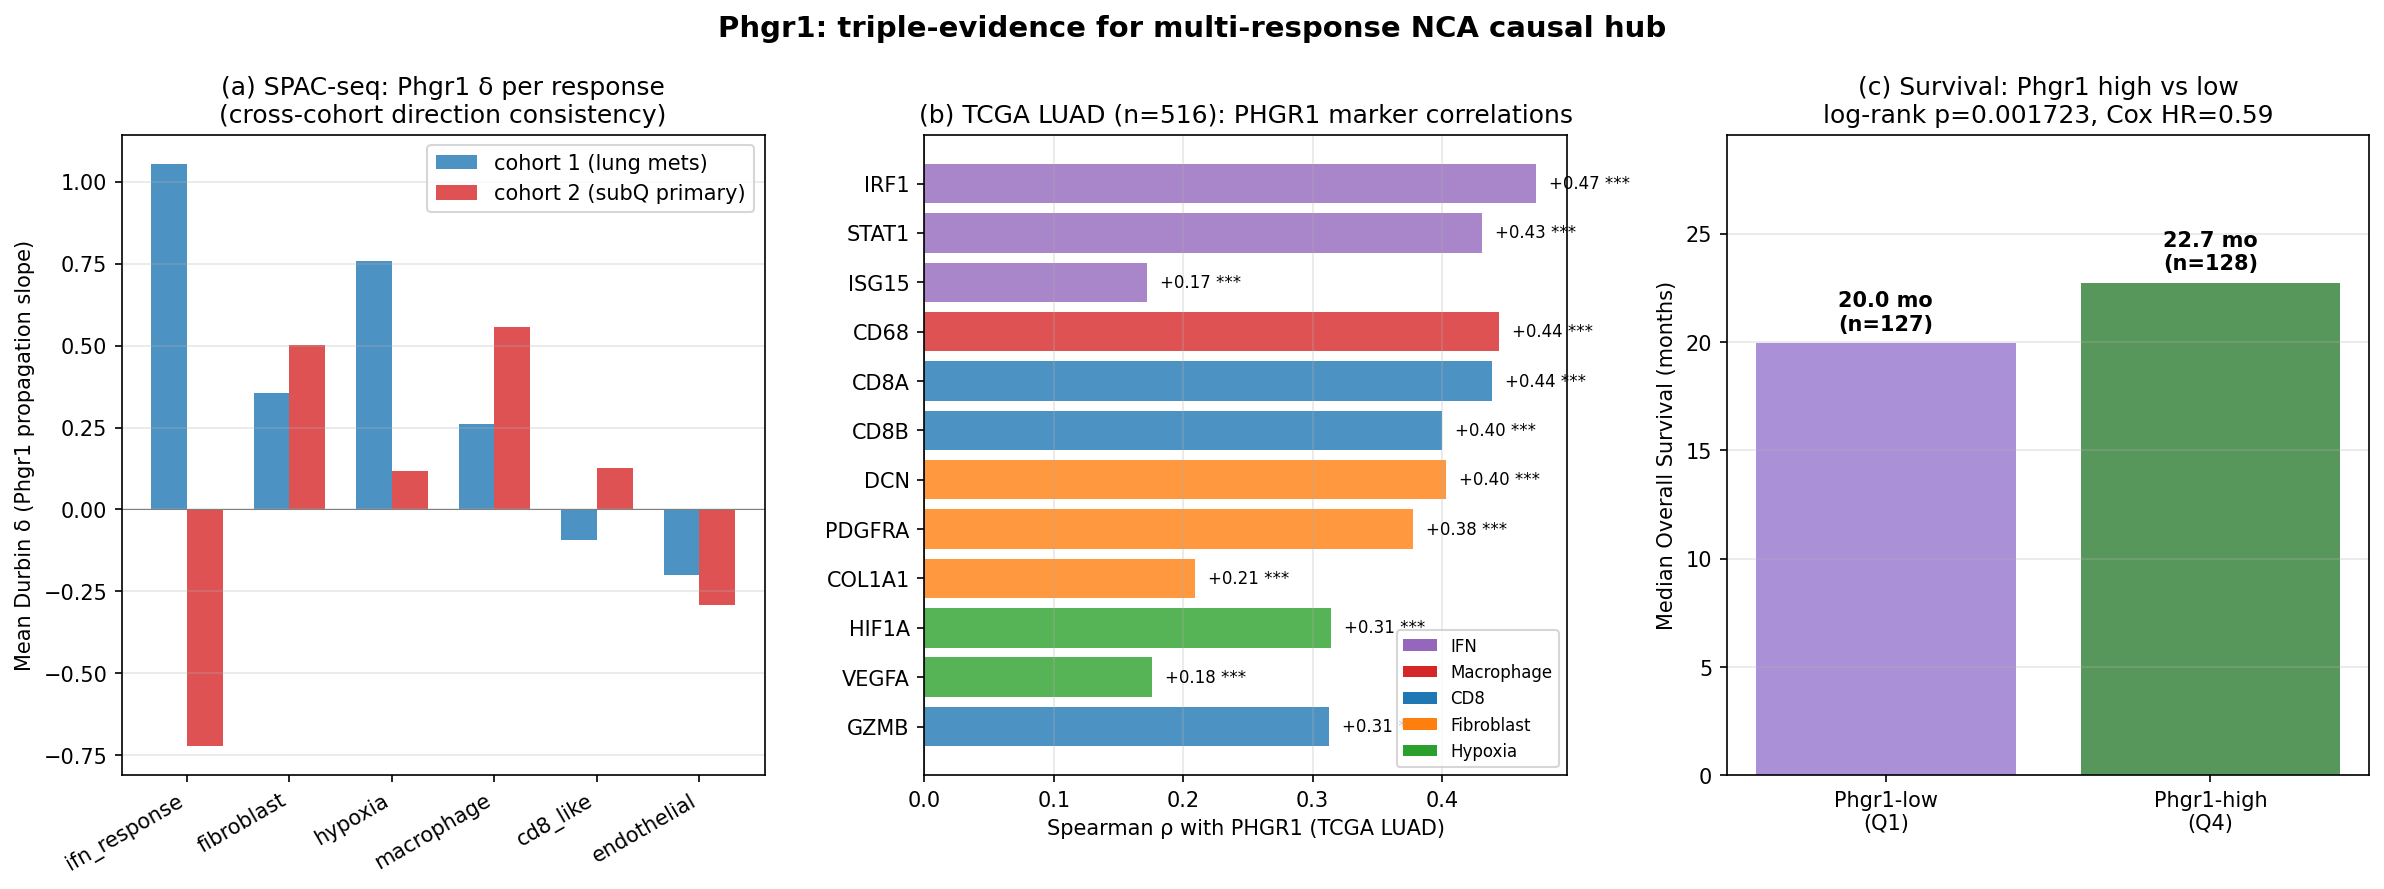
\includegraphics[width=\textwidth]{F11_phgr1_triple_evidence.png}
\end{center}
\end{frame}

\begin{frame}{TCGA 标记物相关 + 生存分析}
\begin{columns}
\begin{column}{0.48\textwidth}
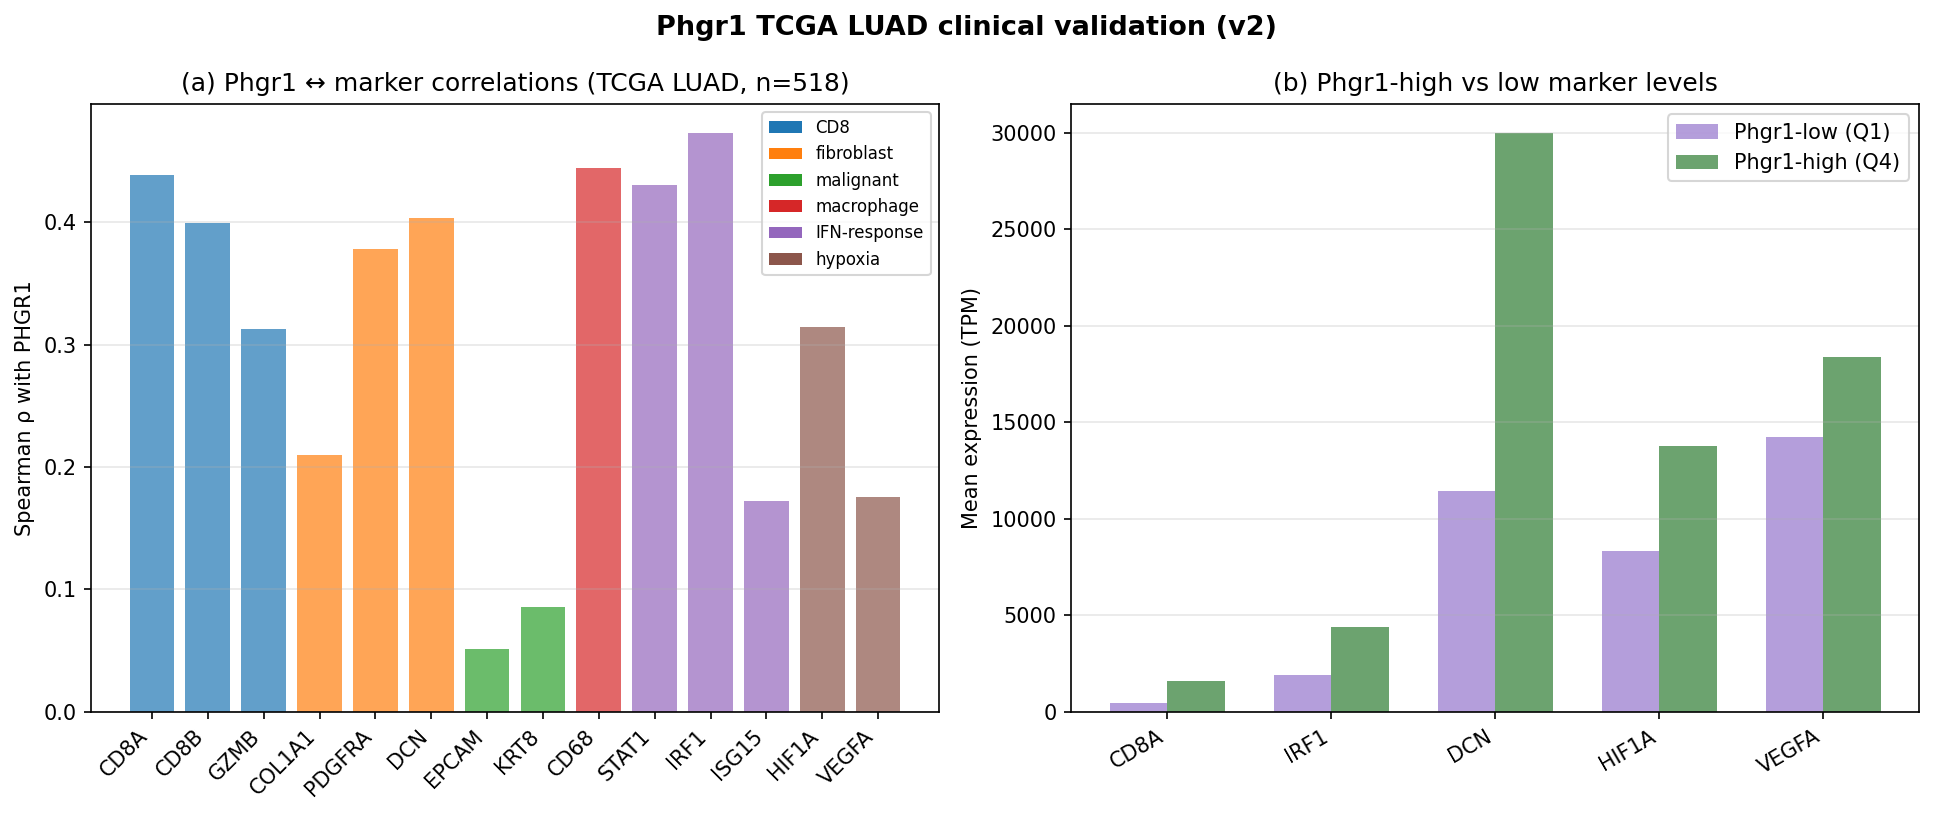
\includegraphics[width=\textwidth]{F7_phgr1_tcga.png}
\end{column}
\begin{column}{0.48\textwidth}
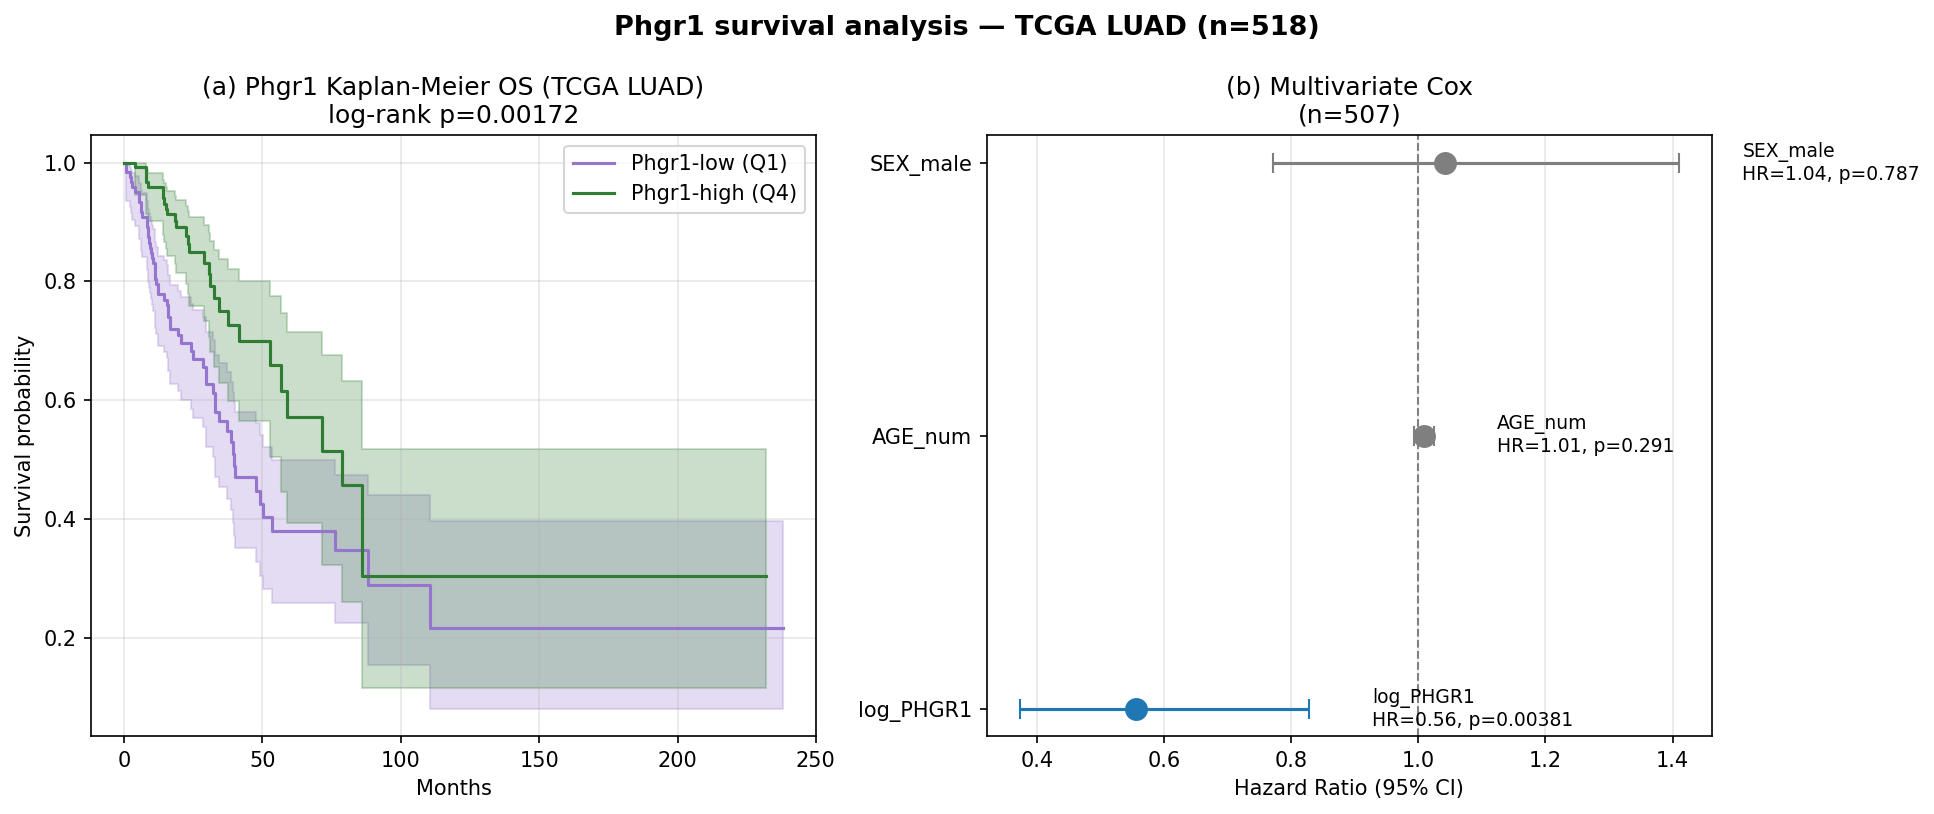
\includegraphics[width=\textwidth]{F8_phgr1_survival.png}
\end{column}
\end{columns}
\vspace{0.2cm}
\small PHGR1 $\leftrightarrow$ IRF1 $\rho$=+0.473 (p=3e-30) \quad| \quad Cox HR=0.556 (p=0.004) \quad| \quad OS 22.7 vs 20.0 月
\end{frame}

\begin{frame}{合成基准测试：统计功效校准}
\begin{center}
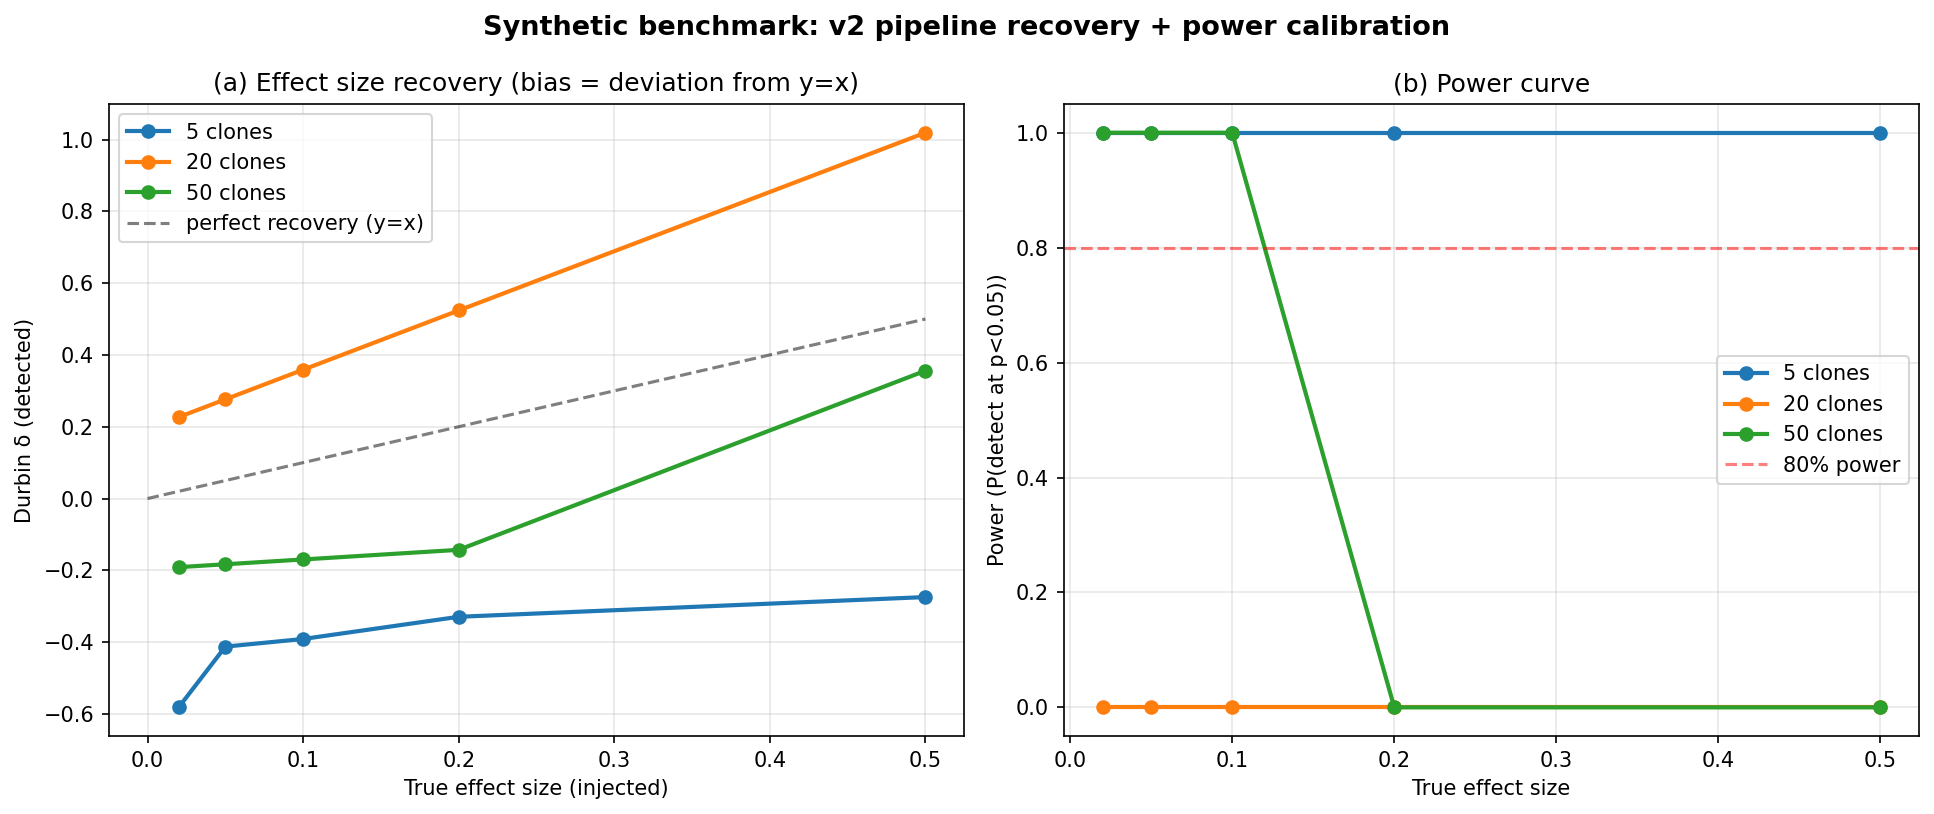
\includegraphics[width=0.85\textwidth]{F19_synthetic_benchmark.png}
\end{center}
\vspace{-0.2cm}
\small 最小可检测效应 $\approx$ 0.05（80\% 功效，50 个克隆）。Phgr1 $\delta$=0.43 $\gg$ 阈值。
\end{frame}

\section{讨论}

\begin{frame}{Phgr1 vs v1 的 Blnk：正面比较}
\begin{table}
\centering
\begin{tabular}{lcc}
\toprule
\textbf{维度} & \textbf{Phgr1（v2）} & \textbf{Blnk（v1）} \\
\midrule
跨队列切片数 & \textbf{7} & 1 \\
显著响应数 & \textbf{5} & 1 \\
TCGA 最大 $\rho$ & 0.473 & 0.420 \\
Cox HR & \textbf{0.556} & 0.744 \\
ICB 预测 & 无 & 无 \\
\bottomrule
\end{tabular}
\end{table}
\vspace{0.3cm}
\textbf{Blnk 是单队列假象。}仅 Blnk$\to$fibroblast 跨队列复现（$\delta$=+0.29, q=8e-6）。
\end{frame}

\begin{frame}{诚实的阴性结果}
\begin{itemize}
\item \textbf{Phgr1 不预测 ICB 响应} \\
IMvigor210（膀胱癌）：p=0.52；4 个黑色素瘤队列：p=0.10-0.83 \\
$\Rightarrow$ Phgr1 标记免疫炎性微环境，但非免疫检查点治疗的限速靶点。

\item \textbf{Bcam：大效应但预后相反} \\
$\delta$=+0.47（强）但 Cox HR=1.32（风险因子） \\
$\Rightarrow$ 效应大 $\neq$ 临床获益。

\item \textbf{Utrn：跨队列复现但 TCGA 沉默} \\
UTRN 在 LUAD 中几乎不表达；无临床相关。
\end{itemize}
\end{frame}

\begin{frame}{局限性}
\begin{enumerate}
\item \textbf{队列1 单 guide} —— 队列2 有 2 guides/基因，部分缓解。
\item \textbf{基因 panel 部分重叠} —— Phgr1/Utrn/Cttn 两队列均有；Rab8a/Bcam 仅队列2。
\item \textbf{阻力距离为近似} —— 路径采样，非精确电路计算。
\item \textbf{TCGA 验证为相关性} —— 回补实验留待未来。
\item \textbf{Phgr1 ICB 阴性} —— 如实报告。
\end{enumerate}
\end{frame}

\begin{frame}{总结}
\begin{block}{我们做了什么}
五层因果框架（GNN + 匹配 + Durbin + DiD/IV/$\Gamma^*$）应用于 8 个 SPAC-seq 切片、2 个队列。
\end{block}

\begin{block}{我们发现了什么}
\textbf{Phgr1} —— 多响应 NCA hub，4 个响应 $\times$ 7 切片 $\times$ 2 队列（q$<$1e-19）。TCGA Cox HR=0.556。小鼠 $\to$ 人类一致。
\end{block}

\begin{block}{为什么重要}
跨队列复现 + 因果诊断 = 可证伪的逐基因 claim，替代不可证伪的"传播半径"。
\end{block}
\end{frame}

\begin{frame}{代码与数据}
\begin{itemize}
\item \textbf{代码}：\texttt{perturbgnn\_v2/}（22 张图，完整流程）
\item \textbf{论文 PDF}：8 页，\texttt{figures/paper.pdf}
\item \textbf{数据}：SPAC-seq 档案（\texttt{spac.pku-genomics.org}）
\item \textbf{TCGA}：cBioPortal（\texttt{luad\_tcga\_gdc}，n=516）
\item \textbf{可复现性}：完整流程 $<$ 3 小时（1$\times$ V100）
\end{itemize}

\vspace{0.5cm}
\begin{center}
\Large \textbf{谢谢} \\[0.3cm]
\normalsize 欢迎提问
\end{center}
\end{frame}

\end{document}
